\documentclass[11pt]{article}

%%%%% Preamble

\usepackage[margin=1in]{geometry} % Margin size
\usepackage{amsmath,amsfonts,amssymb}   % AMS mathematics macros
\usepackage{graphicx}
\usepackage{wrapfig}
\usepackage[export]{adjustbox}

%% Title Information.

\title{\vspace{-1.0cm}JPEG Compression}
\author{Dylan Lathrum}
%\date{October 23 2019} % By default, LaTeX uses the current date

%%%%% The Document

\begin{document}

\maketitle

\section{Introduction}

[Some fancy opening about how data is integral to the information age]
As with everything else, data costs money to store and transfer.
Whether one is looking to store a file on their computer or send an image through the internet, it is often in everyone’s best interest to use as little storage space and bandwidth as possible while still maintaining quality.
This is achieved through compression, a method of reducing the footprint of data by reducing the number of bits needed to represent the data.
Compression methods can be divided into two main categories: lossless and lossy.
Lossless compression is a method where the filesize of the data is reduced without any degradation of the file’s contents; a quality essential to compressing text documents and computer code.
Lossy compression is a more efficient method to reduce file sizes at greater ratios at the cost of losing some detail in the data; a tradeoff that is more acceptable for images and sounds.

Each compression method has their own use cases; for example, it would be a terrible idea to apply a lossy compression algorithm to an essay as some of the data would be lost or changed in the process, while it is perfectly acceptable to run the same algorithm on an image file where the user can afford to lose some detail.
In either case, compression is a trade-off. While some storage space or bandwidth may be saved, something else must be lost.
Whether that be detail in an image, or the processing power required to decompress a file, different algorithms have their strengths and weaknesses.


\section{What is JPEG?}
\label{sec: whatisjpeg}

Specifically, Joint Photographic Experts Group (JPEG) is a lossy compression algorithm that is widely used for images on the Internet.
The entire process that JPEG uses to compress images will be covered in detail, but one of JPEG’s most predominant features is a variable compression ratio.
Most compression methods run at predefined or dynamically generated ratios, making it impossible for a user to choose how compressed they want their data to be.
Because of this, and the algorithm’s efficiency and speed, JPEG has become a standard for digital images.


\section{Preprocessing}
\label{sec: preprocessing}

Before an image can be processed using JPEG, a couple steps are executed to simplyfy the process.
For this paper, the image shown in Figure~\ref{fig:originalImage} will be used at a resolution of 256x138px.
\begin{figure}
  \centering
  \begin{minipage}{0.45\textwidth}
      \centering
      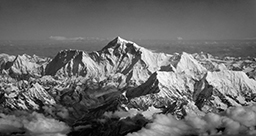
\includegraphics[width=0.9\textwidth]{./images/original.jpg}
      \caption{Original image}
      \label{fig:originalImage}
  \end{minipage}\hfill
  \begin{minipage}{0.45\textwidth}
      \centering
      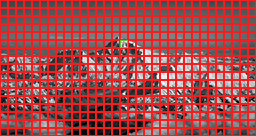
\includegraphics[width=0.9\textwidth]{./images/partitioned_highlight.jpg}
      \caption{Partitioned image}
      \label{fig:partitionedImage}
  \end{minipage}
\end{figure}
The first step is to split the color channels of the image into three distinct grayscale images.
In this example a grayscale picture is used, but in the case of a color image, the image would be split into YCbCr color space, comprised of Luminance (Y), Chroma Blue (Cb) and Chroma Red (Cr), or YCbCr channels.
That way, all calculations are done against three grayscale versions of the image that are recombined at the end of the process.
Once split, image is partitioned into 8x8 chunks as shown in Figure~\ref{fig:partitionedImage}.
This is done to break up the work into smaller chunks to be processed individually.
8x8 chunks are used because blocks of that size often do not have much variance between pixels, and even in larger pictures, these small chunks usually strike the balance between compression ratio and visible artifacts.
This paper will look at the process of compressing one of these blocks, as each block is processed using the same compression method before being stitched back together.

One of the blocks, highlighted in green in above, is shown in detail below.
This is converted into a matrix where each value corresponds to the brightness of the pixel from 0 to 255.
\begin{equation}
  \label{eqn:original}
  
\includegraphics[height = 100pt, valign = c]{./images/block.png}
  \begin{bmatrix}
    243 & 252 & 254 & 251 & 251 & 223 & 164 & 126 \\
    206 & 209 & 245 & 173 & 203 & 255 & 255 & 217 \\
    195 & 180 & 188 & 156 & 161 & 167 & 216 & 243 \\
    160 & 250 & 184 & 146 & 183 & 133 & 109 &  95 \\
    105 & 233 & 143 & 113 & 207 & 140 &  58 &  55 \\
    129 & 209 &  99 & 132 & 239 & 144 &  48 &  54 \\
    221 & 231 & 103 & 129 & 244 & 244 & 124 &  34 \\
    167 & 235 & 111 & 151 & 218 & 214 & 125 &  70
  \end{bmatrix}
\end{equation}

The last step in preparing the data for compression is to subtract each value by 127 in order to center the values around zero.
This ultimately simplifies the math in the following steps by bringing as many values as close to zero as possible.
Now the numbers occupy a range from -127 to 128 inclusive.

\begin{equation}
  \label{eqn:centered}
  P = \begin{bmatrix}
    116 & 125 & 127 & 124 & 124 &  96 &  37 &  -1 \\
    79  & 82  & 118 & 46  & 76  & 128 & 128 & 90  \\
    68  & 53  & 61  & 29  & 34  & 40  & 89  & 116 \\
    33  & 123 & 57  & 19  & 56  & 6   & -18 & -32 \\
    -22 & 106 & 16  & -14 & 80  & 13  & -69 & -72 \\
    2   & 82  & -28 & 5   & 112 & 17  & -79 & -73 \\
    94  & 104 & -24 & 2   & 117 & 117 & -3  & -93 \\
    40  & 108 & -16 & 24  & 91  & 87  & -2  & -57
  \end{bmatrix}
\end{equation}

\section{Transformation}
\label{sec: transofrmation}

Now that the data is in position, calculations can finally be made.
The JPEG format relies on Discrete Cosine Transformation (DCT), which outputs a matrix of weighted coefficients that can be used to represent the 8x8 set of pixels.
Each coefficient corresponds to a separate, predefined cosine function is a certain order.
Figure~\ref{fig:dct} demonstrates the calculated table of cosine functions, and Figure~\ref{fig:dct_order} shows the order that the elements of each 8x8 matrix will be parsed.
\begin{figure}
  \centering
  \begin{minipage}{0.45\textwidth}
      \centering
      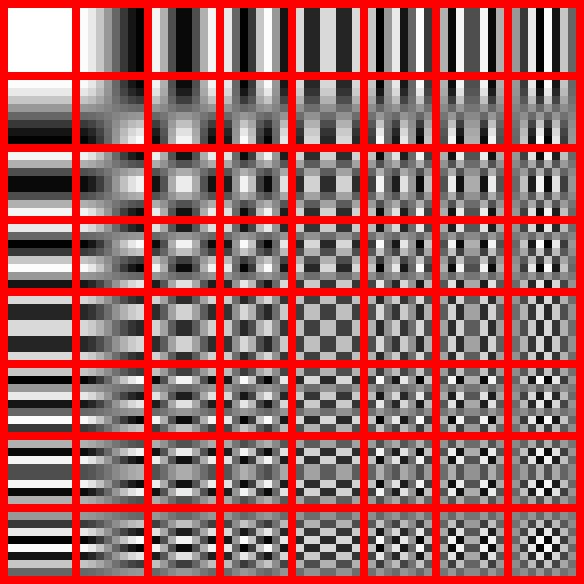
\includegraphics[width=0.9\textwidth]{./images/dct.png}
      \caption{Discrete Cosine Transform}
      \label{fig:dct}
  \end{minipage}\hfill
  \begin{minipage}{0.45\textwidth}
      \centering
      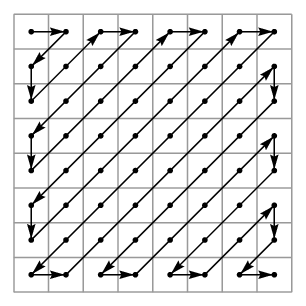
\includegraphics[width=0.9\textwidth]{./images/dct_order.png}
      \caption{Processing order}
      \label{fig:dct_order}
  \end{minipage}
\end{figure}
Thankfully because of this, half of the work is done.
The challenging part is figuring out the coefficients that can be used to create the matrix.
This is achieved using the following function:
\begin{equation}
  \label{eqn:dct}
  X_{u,v} = \alpha(u) \alpha(v) \sum_{x=0}^{7} \sum_{y=0}^{7} g_{x,y} cos \left [  \frac{(2x+1)u\pi}{16} \right ] cos \left [  \frac{(2y+1)u\pi}{16} \right ]
\end{equation}
Where,
\begin{align*}
  &u \text{ is the horizontal index from 0 to 7} \\
  &v \text{ is the vertical index from 0 to 7} \\
  &\alpha(u) \left\{\begin{matrix}
    \frac{1}{\sqrt{2}} & \text{if } u=0 \\ 
    1 &  \text{otherwise}
  \end{matrix}\right. \text{ is a normalizing scale factor to make the result orthonormal} \\
  &g_{x,y} \text{ is the pixel intensity at the coordinents (x,y)} \\
  &X_{u,v} \text{ is the DCT coefficient at the coordinents (u,v)} \\
\end{align*}

\section{Quantization}
\label{sec: quantization}

\section{Compression}
\label{sec: compression}

\section{Decompression}
\label{sec: decompression}

\section{Conclusion}
\label{sec: conclusion}

\section{Further Examples}
\label{sec: furtherexamples}

\bibliographystyle{unsrt}
%\bibliography{bibliography}

\end{document}

